\documentclass[a4paper,12pt]{report}
\usepackage[francais]{babel}
\usepackage[T1]{fontenc}
\usepackage[utf8]{inputenc}
\usepackage{pslatex}
\usepackage{url}
\usepackage{graphicx}
\usepackage{lscape}
\selectlanguage{francais}


\title{Rapport de projet}
\author{
Ihy Group : \\
deguil\_x (Xavier Deguillard)\\
genite\_n (Nicolas Geniteau)\\
sezer\_s (Stephane Sezer)\\
wagnac\_t (Teddy Wagnac)
}
\begin{document}

\maketitle

\section*{Introduction générale}
Dans ce rapport de projet, dédié au codec audio de nouvelle
génération\footnote{en exagérant à peine}, nous essayerons de vous montrer
l'évolution de celui-ci, les impasses que nous avons prises, les choses qui
marchent, celle qui ne fonctionnent pas, etc.\\
Ainsi que vous le verrez dans ce rapport, ce projet doit plus être considérer
comme un sujet de recherche plutôt qu'un véritable nouveau codec. Les
compétences techniques nécessaire à la réalisation d'une telle chose ne sont
vraisemblablement pas à notre portée.\\
Ce rapport sera découpée en plusieurs parties, en premier lieu, la reprise
intégrale du cahier des charges, pour mettre en relief ce que nous voulions
faire et ce que nous avons finalement réalisé. En deuxième partie nous verrons
la chronologie du projet tel que nous l'avons fait. Enfin la dernière partie
A REMPLIR.\\

\tableofcontents

\chapter{Reprise du cahier des charges}
Les pages qui suivent reprennent à l'identique le rapport de soutenance que l'on
vous a rendu en début d'année. Les fautes de
français/orthographe/frappe\footnote{rayez la mention inutile} sont
donc présentes à l'identique.
\documentclass[a4paper,12pt]{article}
\usepackage[francais]{babel}
\usepackage[T1]{fontenc}
\usepackage[utf8]{inputenc}
\usepackage{pslatex}
\usepackage{url}
\usepackage{graphicx}
\usepackage{lscape}
\selectlanguage{francais}


\title{\'Etat de l'art\\Cahier des charges}
\author{
Ihy Group : \\
Teddy Wagnac : \textit{wagnac\_t}, Stéphane Sezer : \textit{sezer\_s},\\
Nicolas Geniteau : \textit{genite\_n}, Xavier Deguillard : \textit{deguil\_x}
}
\date{22 novembre 2008}

\begin{document}

\maketitle

\newpage

\section*{Introduction}
La compression audio est un sujet vaste et les techniques actuelles sont
loin d'être  parfaites.  C'est principalement pour  cela que  pour notre
projet de spé,  qui était totalement  libre,  nous avons choisi un sujet
touchant à la compression audio : la réalisation d'un codec audio.  Dans
la nature,  les  sons ne sont  en fait qu'une  seule et unique  onde que
l'oreille perçoit.  En informatique, la continuité n'existe pas.  Un son
est  en fait  une série  d'échantillons  qui  sont  distant  d'une durée
constante  au  cours  du  temps.   Ces  échantillons  sont  suffisamment
rapproché  pour  que   l'oreille   humaine   ne   détecte   pas  la  non
continuité\footnote{sur  un  CD la  fréquence  des  échantillons  est de
44100Hz}.  On appelle  cela une distribution  discrète.  Tout consiste à
représenter ces  échantillons dans une  forme compressée et  qui ne fait
pas perdre  de qualité (ou  peu) au son  d'origine.  Toute la difficulté
est là.\\
Les premières  techniques de  compression datent  de plus  de 20  ans et
elles ont bien évolué depuis.  Le monde de la compression vidéo et de la
compression audio  étant  liés,  les  innovations  dans  un domaine sont
souvent reportées  dans l'autre avec  une latence plus  ou moins grande.
Un  des  exemples  de  ce  parallélisme  est  l'utilisation  d'un  outil
mathématique particulièrement récent que  l'on nomme les ondelettes.  Il
est utilisé depuis peu dans le traitement des images et de la vidéo,  et
est encore au  stade de recherche pour le  traitement du flux musical.\\
Nous espérons  donc faire ce lien,  en  réalisant un codec  audio qui se
sert principalement des ondelettes.\\
Nous commencerons  donc par  faire un  état de  l'art des  techniques de
compressions,  ainsi  que des  différentes méthodes  d'interactions avec
l'utilisateur, puis enchaînerons sur notre véritable cahier des charges,
dans lequel nous présenterons ce que  nous allons réellement faire et le
planning des différentes soutenances.

\newpage

\tableofcontents

\newpage

\section{\'Etat de l'art}
De façon  très prononcée  dans le  passé,  du fait  des prix  élevés des
espaces de stockages,  et encore aujourd'hui,  du fait de l'augmentation
quasi-exponentielle de la quantité de  donnée que l'on souhaite stocker,
la compression des données sur systèmes informatiques a toujours été une
problématique  importante,  et nombre  de  solutions  ont  été élaborées
jusqu'aujourd'hui.  Nous aborderons ici les  principales pour étudier ce
qui a été fait dans le  domaine de la compression en général,  puis nous
étudierons brièvement  les formats de compression  audio déjà existants.
Nous terminerons alors par un aperçu des différentes méthodes pour créer
une interface homme/machine.

	\subsection{Techniques de compression/décompression}
Nous   aborderons  ici   les  techniques   de  compression/décompression
utilisées   dans  différents   codecs  et   étant  reconnus   pour  leur
performances.

\newpage

		\subsubsection{Compression par ondelettes}
Les ondelettes sont  un outils math\'ematiques apparu il  y a presque 30
ans.  Elles  sont  consider\'ees comme  une  extension  de  l'analyse de
Fourrier.  Au  lieu  de  d\'ecomposer  un  signal  continu  en  somme de
sinusoides,  on le  d\'ecompose en coefficients  \`a partir  d'une autre
base,  pouvant \^etre beaucoup plus compliqu\'e qu'une simple sinusoide.
Le   principal    int\'er\^et   de   cette    technique   est   l'aspect
multi-r\'esolution  de ces  coefficients.  En effet,  les  premiers vont
coder l'aspect g\'en\'eral  du signal puis les autres  vont le d\'efinir
de plus en  plus localement.  Il s'agit d'une  grande am\'elioration par
rapport \`a la transform\'ee de Fourrier.\\
Par exemple prenons un signal contenant certaines asperites locales.  Si
nous   n'avions   pas    cet   aspect   multi-r\'esolution,    celles-ci
influenceraient la quasi-totalite  des coefficients alors qu'ici,  seuls
les  coefficients  locaux   sont  modifi\'es.   Les  ondelettes  peuvent
\'egalement \^etre utilis\'ees sur des  signaux \`a deux dimensions tels
que les images.\\
Pour  le  moment,  la compression  par  ondelettes  est  utilis\'ee dans
plusieurs  algorithmes  de  compression.  Les  deux  principaux  sont le
JPEG2000,  pour les images et le  DIRAC pour les vid\'eos.  En revanche,
il existe  seulement des projets de  recherche concernants l'utilisation
des ondelettes pour la compression du signal sonore.\\
C'est   n\'eanmoins  une   technique   tr\`es   performante   qui  donne
d'excellents r\'esultats  dans  les  domaines  dans  lesquelles elle est
actuellement utilis\'ee.

\newpage

		\subsubsection{Compression fractale}
Peu connue et peu utilisée,  cette compression est souvent associée à la
compression d'images.  Son principe est relativement simple à comprendre
pour un humain, mais l'est beaucoup moins pour un ordinateur.  Il suffit
de  remarquer  sur une  image\footnote{Une  image  permet  de visualiser
rapidement ce  qu'il  se  passe,  contrairement  aux  sons} que certains
motifs se répètent,  ou que certaines parties paraissent très proches au
pour l'œil  humain.  La compression par fractale  va utiliser ceci,  en
quadrillant l'image  deux fois,  l'image source  et l'image destination.
Le maillage de l'image destination doit toujours être plus fin que celui
sur  l'image  source\footnote{Les  fractales  sont  composés  de  motifs
identiques de  plus  en  plus  petit}.  Ensuite,  pour  chaque figure du
quadrillage  source,   on  va  chercher  quelle  figure  du  quadrillage
destination  est  la plus  proche  en  terme  de  contenu(les opérations
mathématiques tels  que  la  rotation  sont  autorisées).  On va ensuite
enregistrer le  couple figure source,  figure destination  ainsi que ses
transformations mathématiques.  En itérant le procédé inverse lors de la
décompression plusieurs fois, on parvient à un résultat très probant.\\
Cette  méthode   présente   plusieurs   avantages   ainsi  que  certains
inconvénient  non  négligeable.  Le  principal  avantage  c'est  que  le
fichier de sortie peut être très  petit,  car il exploite au maximum les
propriété  des  fractales.  Un  autre  avantage  non négligeable,  c'est
l'utilisation pour  l'image source de n'importe  quelle image,  qui doit
néanmoins être présente  lors de la décompression  (un standard pourrait
imposer les  images sources).  De  plus,  de part  la nature  du codage,
l'agrandissement d'une image est  théoriquement possible à l'infini sans
percevoir de  pixels (il  ne faut  pas escompté  non plus  retrouver des
détails  que  l'image  d'origine  n'avait  pas).  Passons  désormais aux
défauts,  le principal souci  vient du fait que les  algorithmes sont de
complexité quadratique  (il faut tester  tous les couples  et trouver le
meilleur), le temps de compression est donc plutôt conséquent.  Un autre
défaut est que l'image reconstituée aura toujours une espèce de flou que
l'on ne pourra enlever qu'en itérant d'avantage.\\
Nous n'utiliserons  pas  cette  compression  pour plusieurs raisons,  la
première est  tout simplement  pour l'un de  ses défauts  : le  temps de
compression,  la  deuxième raison  est que  nous pensons  qu'utiliser la
compression  par  ondelettes  peut-être   beaucoup  plus  instructif  et
intéressant.\\
\begin{center}
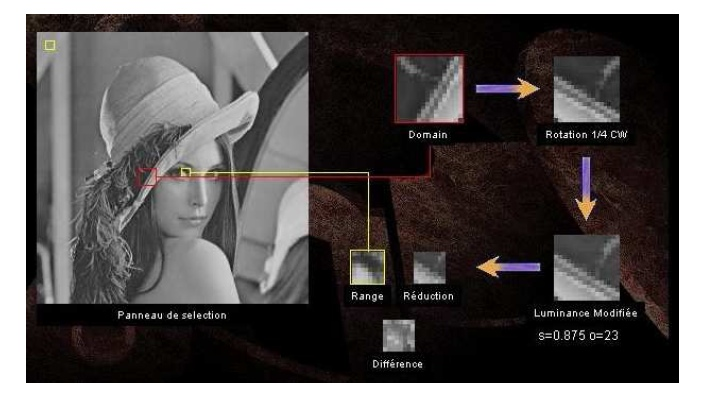
\includegraphics[scale=0.50]{img/compression_fractales.jpg}
\end{center}

\newpage

		\subsubsection{Algorithme de Huffman}
Il s'agit d'un algorithme de  compression sans pertes n'étant absolument
pas spécialisé dans un domaine précis.  Il est notamment utilisé dans le
mp3 ainsi  que dans le  bzip2.  Il utilise un  modèle probabiliste comme
principe de fonctionnement.  En  effet,  l'algorithme d'Huffman tente de
coder les caractères  les plus répandus dans un  fichier avec un minimum
de bits (un caractère est normalement  codé sur 8 bits).  Pour ce faire,
il va tout  simplement compter les occurrences des  256 caractères ASCII
pour établir leur fréquence de  présence.  La phase suivante est la plus
importante,  il s'agit de construire un arbre binaire.  Il faut créer un
nœud pour chaque  caractère et remplir un champ  probabilité pour chacun
des nœuds,  ensuite,  on crée  un nouveau nœud ayant pour  fils les deux
nœuds ayant les probabilités les plus faibles, la probabilité du nouveau
nœud est  tout simplement la sommes  des probabilités de  ses deux fils.
On recommence  le procédé jusqu'à ne  posséder plus qu'un  seul nœud qui
devient la racine de notre  arbre.  Pour déterminer le nouveau code,  on
procède à  la représentation par  occurrences de chaque  élément (qui se
trouvent normalement dans les feuilles).\\
Cette  technique  est extrêmement  efficace  et  c'est  pour  cela qu'on
l'utilisera dans  notre projet.  Il nous  reste à déterminer  si l'on va
faire comme pour  le mp3,  à savoir que la norme  a défini une vingtaine
d'arbre différents,  que  l'encodeur peut utiliser,  il  n'a donc  pas à
reconstruire l'arbre,  ni à l'écrire en début de fichier,  ou à calculer
un arbre adapté au maximum à notre flux en le recalculant à chaque fois.
La première technique possède un inconvénient majeur,  les codages étant
fixés,  ils ne peuvent être optimaux pour toutes les musiques, alors que
la  deuxième  méthode  présente   l'inconvénient  d'utiliser  un  espace
supplémentaire dans  le fichier de  sortie,  et d'imposer des  étapes de
calcul en plus pendant la phase de compression.\\
\begin{center}
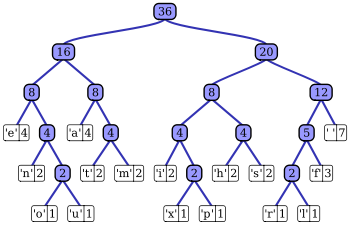
\includegraphics[scale=0.50]{img/huffman_tree.png}
\end{center}

\newpage

		\subsubsection{Transformée de Fourier}
Grand classique en ce qui  concerne la compression,  tant audio que pour
les images,  la transformée  de Fourier permet de passer  du domaine des
échantillons,  au domaines des fréquences.  Cela permet de déterminer le
spectre  d'un  signal,   dans  notre   cas  le  spectre  d'un  son.   En
informatique,  comme  précisé  dans  l'introduction,  les  signaux  sont
représentés sous forme discrète.  Ainsi,  pour représenter un signal, il
faut   considérer  l'ensemble   des  échantillons.   \'A   l'aide  d'une
transformée de Fourier,  le signal peut  être représenté de façon simple
et  compréhensible,  permettant également  la  comparaison  entre codecs
facilement.\\
Nous utiliserons  cette technique  pour plusieurs  raisons.  La première
est que  la  psychoacoustique\footnote{voir  plus  bas} est relativement
simple lorsque l'on travaille sur les transformées de Fourier (il est en
effet très simple de voir les signaux dont la fréquence est supérieure a
15KHz,  fréquence  inaudible  pour  un  humain).  Une  autre  utilité au
transformée de  Fourier,  comme  dit  ci-dessus,  est  la possibilité de
comparer facilement plusieurs flux audio, cela nous servira notamment
lorsque nous comparerons les codecs existant au notre.\\
\begin{center}
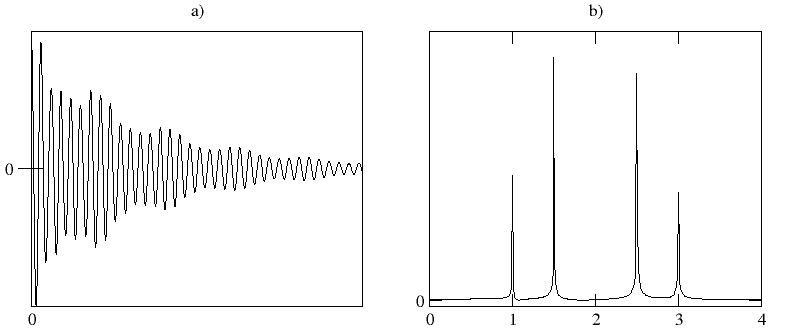
\includegraphics[scale=0.50]{img/transformee_fourier.png}
\end{center}

		\subsubsection{Séries de Fourier}
Il s'agit avant tout d'un outil mathématiques,  extrêmement utilisé dans
le cas d'une  compression audio.  En effet,  un son  n'est rien d'autres
qu'une onde,  malheureusement,  cette  onde n'est  pas simple  à étudier
seule.  Les séries  de Fourier  permettent de se  ramener à  un problème
plus facilement  étudiable.  Elles  permettent  en  effet d'exprimer une
onde complexe comme une  somme de fonctions sinusoïdales,  ainsi l'étude
de  l'onde devient  relativement aisée  et simple.  Toute  la difficulté
réside dans la découverte de ces fonction sinusoïdales ainsi que de leur
coefficients.\\
Nous n'utiliserons  pas cet outils mathématiques  dans notre codec,  les
ondelettes étant une extension des séries de Fourier, nous arriverions à
une certaine redondance.

		\subsubsection{Psychoacoustique}
Très utilisée dans la compression avec pertes, il s'agit d'une étude des
sons,  pour déterminer quels sons sont susceptible de ne pas être perçus
par l'oreille humaine,  ou très  peu entendu.  Par exemple,  on sait que
l'oreille  humaine ne  distingue pas  les  sons  dont  la  fréquence est
supérieure à 15KHz, ou que les basses fréquences sont les mieux perçues.
Grâce à ces  données,  il est assez aisé de  savoir quelles données sont
importantes,  et ainsi,  réduire considérablement la taille d'un fichier
sans  pour  autant  détruire  (selon  la  perception  par  l'oreille) le
signal.\\
Cette technique nous  sera grandement utile car la  réalisation d'un bon
codec audio passe  avant tout par une bonne  connaissance et application
de la psychoacoustique.

\newpage

	\subsection{Codecs audios éxistants}

		\subsubsection{MPEG-1 Layer 1}
Dans le MPEG-1  Layer 1,  le signal brut est découpé  en morceaux de 384
échantillons.  Ces  384 échantillons,  qui  représentent une  trame sont
découpés en  sous-bandes,  et  des  filtres  psychoacoustiques leur sont
appliqués.   On  obtient  ainsi  un  système  de  poids  qui  donne  une
importance plus ou moins grande à chaque sous-bande.  Ensuite, il suffit
d'abaisser la valeur globale de la  quantification tant que la taille ne
correspond pas au débit que l'on souhaite obtenir.\\
Un des gros désavantages de cette méthode est qu'elle ne prend en compte
aucune  technique de  compression lossless  (sans perte)  comme Huffman.
Elle est  en effet adaptée au  systèmes à capacité  très réduite,  et la
rapidité de traitement prime sur la qualité du signal.

		\subsubsection{MPEG-1 Layer 2}
Le MPEG-1 Layer 2,  souvent abrégé mp2 est une étape supérieure entre le
MPEG-1 Layer 1 et le mp3.  Il est toujours très utilisé dans le monde de
la télévision numérique.  Ce codec est très similaire au mp1,  mais il y
apporte quelques  amélioratoins.  Tout d'abord,  le signal  d'entrée est
passé  dans  le   domaine  fréquentiel  et  divisé   en  32  sous-bandes
fréquentielles,  mais dans  le cas du  mp2,  ce sont des  trames de 1152
échantillons qui sont traitées.  De plus, on a la possibilité d'utiliser
3 facteurs d'échelle pour chaque sous-bande.\\
C'est un codec intéressant  qui a eu un grand succès  dans un domaine ou
la simplicité du décodeur était primordiale.

		\subsubsection{Le mp3}
Le  mp3 apporte  nombre d'améliorations  comme  par  exemple  les trames
produites  sont  de  taille  variables  ce  qui  permet  de  privilégier
l'utilisation  de l'espace  disponible pour  les  passages  ou  une plus
grande précision est requise.\\
De plus, le mp3 fait usage de techniques de compression sans perte après
avoir utilisé un modèle psychoacoustique, tels que Huffman.\\
Le succès du mp3 est incontestable au  vu de sa très grande présence sur
le marché de l'audio numérique.

		\subsubsection{Vorbis}
Le vorbis (g\'en\'eralement  connu sous le nom de ogg  vorbis du fait de
son  conteneur  standard),  est  un  codec  audio  plus  recent  et plus
performant que le mp3, mais est encore moins repandu que ce dernier.  Il
est r\'ealis\'e  au sein de la  fondation xiph.org et est  libre de tout
brevet.\\
Il  utilise   des  techniques  de  compression   similaires  \`a  celles
utilis\'ees pour le jpeg et le MPEG, c'est \`a dire des algorithmes avec
perte  qui   se  basent  sur   l'etude  de  la   perception  humaine  de
l'information.\\
Son avatange qui est aussi un d\'esavantage : il utilise des algorithmes
r\'ecents et plus complexes.

\newpage

	\subsection{Interface homme/machine}
		\subsubsection{Qt}
Principalement  utilisé  dans  l'environnement  de  bureau  KDE  sur les
systèmes UNIX,  mais utilisable  à la fois sur Windows que  sur Mac OS X
ainsi que pour l'environnement de bureau Gnome,  Qt est une bibliothèque
logicielle permettant de faire  une interface graphiques.  Son principal
avantage est son extrême portabilité,  en effet,  le même code peut être
compilé sur Windows  et UNIX.  Le résultat est bien  évidemment le même.
Son principal  défaut (pour nous  utilisateur de  l'environnement Gnome)
est qu'il s'intègre mal à cet environnement de bureau.\\
De plus, Qt est codé en C++ et pas en C, et notre projet doit uniquement
faire sage du C et de l'Ocaml.  Pour ces raisons,  nous ne l'utiliserons
pas.\\
\begin{center}

\includegraphics[scale=0.50]{img/qt.png}
\end{center}

		\subsubsection{GTK}
GTK+ (The Gimp  Toolkit) est un ensemble de  bibliothèques permettant de
réaliser  des interfaces  graphiques.  Il est  surtout utilisé  pour des
projets comme les environnements de bureau GNOME ou encore ROX.\\
GNOME (GNU  Network Object  Model Environment)  est un  environnement de
bureau libre convivial;  cette interface  est actuellement populaire sur
les  systèmes  GNU/Linux et  fonctionne  également  sur  la  plupart des
systèmes de type UNIX.  ROX Desktop est un environnement de bureau libre
pour  Unix.  Il est  basé sur  le  gestionnaire  de  fichiers ROX-Filer.
C'est un  logiciel libre distribué selon  les termes  de la  licence GNU
GPL.\\
C'est un  ensemble  de  bibliothèques  logicielles  libre.  On peut donc
l'utiliser  entièrement  dans  les  conditions  de  la  licence,  il est
totalement compatible avecun environnement de type BSD et est utilisable
avec le langage C.\\
Grâce à  GTK+,  nous espérons  réaliser une  interface de  lecteur audio
complète et  interactive.  Et nous  utiliserons la  version 2.0  qui est
plus récente et offre plus de possibilités que la précédente.\\
\begin{center}

\includegraphics[scale=0.50]{img/GTK.png}
\end{center}

		\subsubsection{La Console}
La console,  véritable boîte à outil de l'utilisateur d'UNIX,  permet de
tout faire,  de la  lecture de mail au surf sur  internet en passant par
des  lecteurs  musicaux et  des  lecteurs  pdf.  De  plus,  la  ligne de
commande est uniforme pour tous  les systèmes UNIX,  c'est LE gros point
commun.   Une   application  se   doit   donc   d'avoir   une  interface
texte\footnote{les barbus  peuvent ainsi utiliser  nos logiciels sans
avoir à installer d'interface graphique}.  De plus,  avoir une CLI
permet souvent de  travailler de façon plus efficace,  par
exemple  en  faisant des  scripts  qui  vont  convertir  l'ensemble d'un
répertoire au format  ihy,  ce qui est rarement faisable  à l'aide d'une
interface graphique.\\
Cette interface non graphique nous  permettra donc dans un premier temps
de  tester que  le codec  fonctionne et  dans un  second temps  de faire
plaisir à nos amis les barbus.

\newpage

\section{Cahier des charges}

	\subsection{Présentation du projet}
Le projet Ihy  a pour ambition d'utiliser l'outil  mathématique que sont
les ondelettes pour  compresser du son.  Elles sont  déjà utilisées dans
le domaine de  l'image et de la vidéo,  mais  pour l'audio,  les projets
n'en  sont  qu'au  stade  d'ébauche  et  de  recherche.  Le  travail  se
focalisera  sur  le  traitement  de  fichiers  musicaux.  Une  recherche
mathématique devra être portée,  pour trouver les bonnes ondelettes,  et
plus  précisément  celles  adaptées  au   format  de  fichier  que  nous
traiterons.  En  effet,  comme  dans  tout  algorithme  de  compression,
certaines variables dépendent du type de donnée à traiter.\\
Le projet sera donc axé sur l'élaboration de ces algorithmes,  ainsi que
la reprise d'autres,  déjà existants  comme Huffman pour des traitements
en plusieurs passes.\\
Le projet comprendra  également un lecteur pensé  spécifiquement pour le
format ihy mais qui devra tout de même rester indépendant des librairies
de compression  décompression du projet.  En  effet,  si nous souhaitons
redistribuer notre format par la suite,  il  est préférable de ne pas le
lier  à   un  lecteur,   ce  qui  compliquerait   la  tâche  d'éventuels
utilisateurs de notre code.\\
Le lecteur comprendra des fonctions très simples (lecture/pause,  avance
rapide  et  retour  arrière)  ainsi  qu'un  éventuel  spectrographe  qui
enjolivera le tout  en  offrant  des  effets  de  visualisation les plus
plaisants possibles.\\
Une partie non négligeable du travail,  abordée précédemment, sera l'API
qui servira  d'interface  au  monde  extérieur.  Nous  devrons suivre un
certain nombre de règles pour permettre une utilisation du format ihy la
plus répandue et efficace possible.

	\subsection{Ihy Group}
Le ihy  group est l'équipe  qui va s'atteler  à la tâche  de réaliser ce
nouveau format  de compression audio ainsi  que le  lecteur qui  lui est
associé.  Chacun des membre est présenté dans la section suivante.\\
Quant au nom du groupe,  il provient d'une divinité égyptienne : le dieu
Ihy,  qui était  fils d'Hathor,  dieu de  la musique et  du sistre.  Son
rapport  avec   la  musique   et  l'imprononçabilité   du  nom   nous  a
immédiatement séduits, et c'est ainsi qu'a démarré le Ihy group.

	\subsection{Présentation des membres}

		\subsubsection{Stéphane Sezer}
Stéphane Arsène  Sezer est un  étudiant d'epita évoluant  en Spé A2.  Il
faisait partie  l'année passé du  Heenok Crew et  était même chef  de ce
projet apprécié par tout ceux qui ont pu le tester.  Dans ce dernier, il
s'est occupé du réseau ou encore du site web.\\
Aujourd'hui,  il fait partie à part entière du ihy group,  où il a gardé
son statut de chef de projet car il a bien mené son équipe l'an passé et
pense qu'il sera aussi performant, voir plus encore cette année.\\
Arsène sera chargé de compresser les morceaux de musique grâce notamment
au  développement  du  principe  des  ondelettes  et  une  étude  de  la
psychoacoustique.

		\subsubsection{Xavier Deguillard}
Lui aussi  a eu la  chance de travailler sur  le projet "La  course à la
gazoline"  avec le  Heenok Crew,  où  il fut  un élément  essentiel pour
l'équipe.  En effet, il a touché un peu à tout dans le projet mais était
personnellement  chargé  du moteur  graphique  (qui  fut  la  plus belle
réussite du projet).\\
Maintenant,  il a rejoint le ihy group pour lequel il va mettre en avant
son savoir et sa détermination inégalée à ce jour.\\
Et  donc,   Xavier  sera  personnellement   chargé  des  algorithmes  de
compression annexes,  des connexions des  différents éléments entre eux,
de l'API et apportera son soutien dans le domaine de la psychoacoustique
également.

		\subsubsection{Teddy Wagnac}
Teddy Wagnac est  un  jeune  étudiant  d'epita  évoluant  en Spé B2.  Il
faisait partie l'année dernière du fameux Heenok Crew qui prônait gloire
et  allégeance au  Roi Heenok,  artiste  incontesté de  la scène  rap au
Canada,  et a donc  participé  grandement  au  développement  du jeu "la
course à la gazoline" où il  était chargé de différentes tâches comme le
moteur physique ou encore l'aide du jeu.\\
Mais maintenant,  il  forme le ihy  group,  et avec ses  trois camarades
compte bien  réaliser un projet plus  sérieux que  celui de  l'an passé.
Pour  sa  part,  il  sera  chargé  entre  autre  de  la  réalisation  de
l'interface graphique et du spectrographe.

		\subsubsection{Nicolas Geniteau}
Seul membre du  groupe qui ne faisait pas partie  du Heenok Crew l'année
dernière,  Nicolas Geniteau  a rejoint  Xavier,  Stéphane et  Teddy pour
permettre l'élaboration  d'un codec d'un genre  nouveau.  Il nous aidera
avec ses connaissances en caml et ses talents de geek presque barbu.\\
Son sérieux  et son  assiduité feront  sûrement de  lui un  élément très
utile à l'avancée du projet.

	\subsection{Répartition des tâches}
\begin{itemize}
	\item Stéphane Sezer : écriture des  algorithmes de
compression/décompression par les ondelettes, et travail sur la
psychoacoustique, site web.
	\item Nicolas Geniteau : écriture des algorithmes de
compression/décompression en ondelettes.
	\item Teddy Wagnac : interface en GTK (et SDL pour un possible
spectrographe), lecture du son.
	\item  Xavier  Deguillard  :  algorithmes  de  compression  annexes,
	connexion des différents éléments entre  eux,  API et travail sur la
	psychoacoustique.
\end{itemize}

\newpage

	\subsection{Taches à accomplir}

		\subsubsection{Travail sur les ondelettes}
Cette partie est la pierre  angulaire du projet.  L'étude des ondelettes
ainsi que la recherche de celle ou celles qui sont les mieux appropriées
à la compression du signal sonore  va demander un temps non négligeable,
c'est pourquoi  deux membres  du groupe se  chargeront de  cette partie.
Ces deux membres sont Nicolas et Stéphane.\\
Cette partie  peut  elle-même  être  divisée  en deux sous-sections.  La
première est  la recherche en  tant que telle,  se  rapprochant plus des
mathématiques que de  l'informatique,  la seconde étant l'implémentation
des résultats  précédemment  trouvés.  Cette  implémentation  se fera en
OCaml,   c'est  un   langage  particulièrement   adapté  pour   ce  type
d'opérations car c'est un langage  fonctionnel,  et nous allons bien sûr
travailler sur des fonctions mathématiques.

		\subsubsection{Algorithmes annexes}
Les ondelettes  sont très  intéressantes,  mais elle  ne sont  pas grand
chose  sans l'utilisation  de procédés  supplémentaires pour  réduire la
taille  des  informations.   Nous  utiliserons  donc  très  probablement
l'algorithme  d'Huffman  en  seconde  passe  et  peut-être  du RLE.  Ces
algorithmes  restent particulièrement  simples,  mais il  faudra étudier
leur efficacité selon leur position  dans la file de traitement,  et ils
deviendront donc intrinsèquement plus difficiles à manipuler.\\
Huffman et RLE ne  sont que deux exemples de ce que  Xavier sera amené à
aborder dans cette  étude.  Il est également probable  que nous fassions
usage des outils  comme  la  transformée  de  fourrier  pour analyser la
répartition fréquentielle de notre échantillonage et permettre ainsi une
étude psychoacoustique du flux.\\
Ces algorithmes seront écrits en C ou en OCaml, avec une préférence pour
l'OCaml, étant donnée la nature mathématique de la tâche à accomplir.

		\subsubsection{Psychoacoustique}
La  psychoacoustique   est  toujours  une  partie   importante  de  tout
algorithme  de  compression  audio  avec  perte.  Dans  le principe,  la
psychoacoustique étudie la manière  dont l'information sonore est captée
par le système  auditif  et  comment  elle  est  traitée par le cerveau.
Toute la subtilité se trouvant  dans le fait d'utiliser ces informations
pour éliminer ou estomper les informations les moins prépondérantes dans
le flux  audio.  Un des résultats les  plus simples  à traiter  reste le
fait que l'oreille humaine ne peut entendre les sons qui sont hors de la
plage de fréquence qui s'étend de 20 à 15 000Hz.\\
Les ondelettes,  précédemment  citées,  peuvent éventuellement effectuer
une partie du  travail qui est réservée à  la psychoacoustique,  mais il
faut aussi  prendre en compte  l'efficacité des algorithmes,  et  il est
possible que pour certains cas,  il  soit plus avantageux d'utiliser des
algorithmes plus "traditionnels".

		\subsubsection{Lecteur / Interface graphique}
Le lecteur peut être vu comme  un mini-projet séparé de l'élaboration du
codec.  C'est Teddy qui  se chargera de tout ce  travail en apportant un
soin particulier à  l'interface  et  à  l'apparence  qui  est un élément
important pour l'utilisateur final.  En effet,  le lecteur utilisera des
fichiers  binaires  (probablement  des  .so)  fournis  par  les  travaux
précédents pour fonctionner.  La présence d'un lecteur associé au projet
mais totalement  modulaire  a  l'avantage  de  permettre à l'utilisateur
final de  tester notre format sans  grande complication,  mais permettra
quand même  une réutilisation du  codec,  détaché de  son lecteur,  dans
d'autres projet.\\
L'interface graphique permettra aussi de tagger ses fichiers musicaux en
y entrant les métadonnées que l'on  souhaite ajouter.\\ Comme on peut le
voir,  la modularité est le maître mot qui guide toute l'organisation de
notre  travail.  Cette modularité  permettra  l'établissement  d'une API
standardisée.\\
Cette partie  sera entièrement faite  en C,  premièrement parce  que les
librairies GTK sont  en  C,  et  deuxièmement  parce  que l'OCaml semble
relativement peu adapté à l'établissement d'une interface graphique.

		\subsubsection{L'API}
L'API  n'est  pas  une  tâche  en  elle-même.  Elle  comprend  en  effet
plusieurs règles  à respecter,  comme la modularité  du code,  ainsi que
l'établissement de  spécification strictes expliquant  le fonctionnement
de la  compression,  de la décompression,  ainsi  que du  conteneur qui,
comparable à l'ogg, pourra éventuellement être réutilisable.\\
Il faudra  tout de  même penser à  la création  de binaires  d'un format
particulier,  et gérer  toutes les règles  d'un Makefile  pour accomplir
cette tâche.  Un soin particulier à  l'assemblage des éléments entre eux
sera aussi apporté par Xavier pour la réalisation de cette partie.

		\subsubsection{Site Web}
Pour ce type de projets,  le site  web est incontestablement le moyen de
communication  le   plus  répandu.   Nous  en   aurons  donc   un  dédié
spécifiquement  à  notre projet  avec  un  repository  svn  associé pour
permettre le travail collaboratif.\\
Il sera disponible à l'adresse \url{http://thrashboul.com/ihy}\\
Le    d\'ep\^ot    svn   sera    quant    \`a    lui    disponible   sur
\url{http://thrashboul.com/ihy/svn}

\newpage

\begin{landscape}
	\subsection{Planning}
	\begin{center}
	\begin{tabular}{||l||c|c|c||}
		\hline
		\hline
		Élément & Soutenance 1 & Soutenance 2 & Soutenance finale \\
		\hline
		\hline
		Compression   ondelettes   &   Commencé   (encodage)   &  Avancé
		(compression) & Terminé \\
		\hline
		Lecture  du fichier  ihy &  Différentes  sections  &  Commencé &
		Terminé \\
		\hline
		Algorithmes annexes & Commencé & Avanc\'e & Terminé \\
		\hline
		Interface / Lecteur & Commenc\'e & Avancé & Terminé \\
		\hline
		Site web & Terminé & Terminé & Terminé \\
		\hline
		\hline
	\end{tabular}
	\end{center}
\end{landscape}

\newpage

\section*{Conclusion}
L'aventure  dans  laquelle  se  lance  le   Ihy  group  est  à  la  fois
intéressante sur  le plan  algorithmique que  sur le  plan mathématique.
Elle permettra comme tout travail en groupe d'apprendre à coordonner ses
efforts avec  ses compagnons  pour arriver  à donner  le meilleur  et la
satisfaction que peut  procurer la réussite d'une  telle entreprise sera
une récompense non négligeable de ces efforts.\\
Voilà comment l'équipe du Ihy group compte créer un codec audio afin que
tout individu  puisse savourer le  bonheur d'écouter de  la musique avec
une compression  du son  qui frôle  la perfection.  En  effet,  on parle
souvent du bonheur  des  yeux  ou  encore  des  papilles mais on néglige
systématiquement celui  de l'ouïe  en se  contentant de  sons compressés
hideusement.  Pour cela,  l'équipe  présentée  précédemment  composée de
Stéphane Arsène Sezer,  le chef  du groupe généreux et impliqué,  Xavier
Deguilard déterminé et talentueux,  Nicolas Géniteau ingénieux et motivé
et enfin Teddy Wagnac plein de  bonne volonté et dynamique vont associer
leurs  connaissances et  leurs ingéniosités  pour arriver  à bout  de ce
projet qui  leur tient à cœur  et qui  les passionne.  C'est  donc plein
d'espoir et d'ambition que le Ihy  group entame ce projet qui vise toute
personne intéressée par  la musique en général et est  déçue de voir ses
morceaux favoris gâchés par une compression  qui se préoccupe plus de la
taille du fichier  final  que  de  la  qualité  sonore.  Il faut arrêter
d'offenser nos  pauvres oreilles et le  Ihy group et la  pour les sauver
cette torture infernale.

\end{document}


\chapter{Chronologie du projet}
\section{Première soutenance}
\subsection{L'état du codec}
Il faut le dire, le codec audio n'était pas très utile à cette époque. En effet,
celui-ci ne compressait pas la musique, au contraire, il doublait la taille du
fichier wav original non compressé. En effet, nous passions d'un échantillons
codé sur 2 octets dans le cas du wav, à un coefficient d'ondelettes codé sur 4
octets. Les données écrites étant brutes, cela doublait effectivement la taille
du fichier.\\
Si l'on excepte ce petit défaut, nous pouvions encoder un fichier ihy, le
décoder pour obtenir le fichier original. Cela a montré plusieurs choses,
premièrement, que les ondelettes que nous avions implantés fonctionnent,
deuxièmement, que l'interface entre le C et le Caml fonctionne également, et
enfin, que notre fichier ihy est parfaitement lisible, et l'on peut donc en
extraire sans problèmes les informations dont on a besoin.\\
Les techniques de compression utilisées étaient inexistantes, la compression via
l'algorithme de Huffman avait été implanté, mais pas sa décompression. Quand aux
ondelettes, nous avions implantés l'ondelette la plus simple de toute (mais
néanmoins très puissante), qui est l'ondelette de Haar.\\
De plus, nous pouvions lire un fichier wav et utiliser la carte son de
l'ordinateur pour lire le fichier wav en question, ceci afin de préparer la
lecture d'un fichier ihy en lui-même que nous n'avions pas à cette soutenance.
\subsection{L'interface graphique}
Lors de cette première soutenance, notre interface graphique était des plus
sobre, elle n'était constitué que de 5 boutons, ainsi que d'une barre de
progression. Cette dernière se remplissait lorsque l'on appuyait sur le bouton
``play'', afin de simuler l'avancement d'une musique.
\subsection{Ce que nous ne savions pas}
L'informatique n'est pas une science exacte, et nous avons pu le vérifier après
cette soutenance. En effet, le fichier décompressé étant le même (à l'oreille),
nous ne nous doutions pas qu'il y avait un problème. En fait, 75\% des
coefficients d'ondelettes n'étaient pas présent dans le fichier ihy, ils étaient
remplacés par des caractères ``random'', la faute à un memcpy dont la taille à
copié avait été mal renseignée.\\
Néanmoins cette petite erreur nous a appris une chose, les ondelettes sont un
outil puissant qui avec un peu de travail peuvent donner naissance à un codec
audio très intéressant\footnote{En réécoutant attentivement le fichier wav en
sortie, ce dernier était au final assez différent de l'original.}.
\subsection{Conclusion partielle}
Une bonne première soutenance donc, qui nous a permis de nous familiariser avec
les ondelettes ainsi qu'avec le développement sous UNIX en C et Caml.

\end{document}
